\section [Xylene degradation (1D)]{1D reactive transport: Xylene degradation with multiple monod kinetics, exchange kinetics and biomass growth}
\label{l_s_benchmark_1d_xylene_deg}

\subsection{Definition}
This benchmark describes the reactive transport of xylene in a homogeneous aquifer. The main purpose is to document the ongoing reactions, which are xylene degradation under aerobic, sulfate reducing and iron reducing conditions, considering growth of the respective biomasses. Also included is the rate limited exchange of iron goethite into bioavailable iron. The aquifer is represented by a one-dimensional model of 50 m length in the x-direction and 1 m in the y-and z directions, respectively. The model is discretized by 100 line elements of constant 0.5 m length in x direction. With an isotropic hydraulic conductivity K of 2.13 $\times$10$^{-3}$ m s$^{-1}$, a porosity of 0.24 and a hydraulic gradient I of 1.3$\times$10$^{-4}$, the steady state transport velocity va is 0.1 m d$^{-1}$. Longitudinal dispersivity  $\alpha_L$ is set to 0.25 m, the diffusion coefficient $D_a$ is set to 1.0$\times$10$^{-9}$ m$^2$ s$^{-1}$. The physical aquifer parameters are summarized in Tab.~\ref{l_tab_benchmark_1d_xylene}. The transport simulation is run for a period of 1000 d with a time step length of 5 d.

The model aquifer has a length of 50 m in the x-direction, 1 m in the y-direction and 1 m in the z direction. The whole domain is discretized into 100 line elements with a constant x and y dimension of 1 m.
The aquifer is assumed to have a homogeneous and isotropic hydraulic conductivity. Using a gradient of 1.23 $\times$10$^{-4}$ and a porosity of 0.24 produces a steady state transport velocity of 0.10 m d$^{-1}$.Xylene degradation is simulated according to the typical redox sequence.


\begin{table}[htbp]
\caption{Parameters used for benchmark HC$\backslash$1d\_xylene\_degradation }
\centering
\begin{tabular}{|l|l|l|}
\hline
Parameter & Value & Unit \\
\hline
porosity $\Phi = n $  & 0.24 &  --  \\			
matrix volume fraction $VOL_MAT $  & 0.75 &  --  \\			
biomass volume fraction $VOL_BIO $  & 0.01 &  --  \\			
hydraulic conductivity $K$ & 2.13$\times 10^{-3}$ & m$\cdot$s$^{-1}$ \\
storage coefficient $S$ & 0.0 & s$^{-1}$ \\
solid density $\rho_s$ & 2000 &  kg$\cdot m^{-3}$ \\
density of water $\rho_w$ & 1000 & kg$\cdot m^{-3}$ \\
viscosity water $\eta$ & 0.001 & Pa$\cdot s$ \\
longitudinal dispersivity $\alpha_l$ & 0.25 & m \\
component diffusion coefficient $D$ & 1.0$\times 10^{-9}$ & m$^2 \cdot$ s$^{-1}$ \\
\hline
\end{tabular}
\label{l_tab_benchmark_1d_xylene}
\end{table}

Model results are compared an older version of \GeoSys.

\subsection{Solution}

Results of the simulation are shown in Fig.~\ref{profiles_xylene_degradation} for xylene, the electron acceptors oxygen and sulfate, as well as for the biomass of the aerobic microorganisms, the sulfate reducers and the iron reducers simulation time steps of 100 days.
For simulation time t $<$ 500~d, one can see the advancing xylene front, a reduction of xylene concentrations is only visible for later times, when xylene concentrations reduce to about 90\% of the inflow concentration. Also shown is the increasing consumption of oxygen with time, accompanied by the growth of the aerobic reducers at the inflow (left) end of the model area. After approximately 800~d, oxygen concentrations in the inflowing groundwater are reduced to almost zero within the first 20~m of the aquifer. Sulfate reducers initially decay from their initial amount, as growth is inhibited throughout the column by the still high concentrations of oxygen. Once oxygen is used up, however, sulfate reducers start to grow downstream of the oxygen reducers and sulfate concentrations in the groundwater reduce accordingly. The iron reducers decay from their initial values and start to grow only for late times t $>$ 80~d and x $>$ 30~m, as xylene degradation from iron reduction is inhibited by both, oxygen as well as sulfate, which is still present in concentrations larger than the inhibition concentration for iron reducers. Accordingly, the spatial distribution of bioavailable iron is still almost uniform throughout the aquifer.


\begin{sidewaysfigure}
\centering
\includegraphics[width=0.9\textwidth]{PART_III/HC/profiles_xylene_degradation.eps}
\caption{Profiles of oxygen, sulfate and xylene (top row, from left) and  aerobic reducers, sulfate reducers and iron reducers at different times during the 1000 d simulation period.}
\label{profiles_xylene_degradation}
\end{sidewaysfigure}
